\documentclass[preview]{standalone}

\usepackage{amsmath}
\usepackage{amssymb}
\usepackage{stellar}
\usepackage{definitions}
\usepackage{bettelini}
\usepackage{tikz}

\begin{document}

\id{graph-walks-connectedness}
\genpage

\section{Walks and paths}

\begin{snippetdefinition}{walk-definition}{Walk}
    Let \(G\) be a \graph.
    A \emph{walk} in \(G\) is a finite alternating sequence of vertices and
    edges
    \[
        v_0,e_1,v_1,e_2,v_2,\ldots,e_n,v_n
    \]
    such that, for every \(i=1,\ldots,n\), the endpoints of \(e_i\) are
    \(v_{i-1}\) and \(v_i\).
    The vertices \(v_0\) and \(v_n\) are called the \emph{origin} and the
    \emph{terminal vertex} of the walk.
\end{snippetdefinition}

\begin{snippetdefinition}{trail-definition}{Trail}
    Let \(G\) be a \graph.
    A \emph{trail} in \(G\) is a \walk in which no edge is repeated.
    Vertices are allowed to repeat.
\end{snippetdefinition}

\begin{snippetdefinition}{path-definition}{Path}
    Let \(G\) be a \graph.
    A \emph{path} in \(G\) is a \walk in which no vertex is repeated.
\end{snippetdefinition}

\begin{snippetdefinition}{cycle-definition}{Cycle}
    Let \(G\) be a \graph.
    A \emph{cycle} in \(G\) is a closed walk
    \[
        v_0,e_1,v_1,\ldots,e_n,v_n
    \]
    whose only repeated vertex is \(v_0=v_n\).
\end{snippetdefinition}

\begin{snippet}{walks-paths-illustration}
    The same graph may contain many walks, trails, paths, and cycles:
    \[
        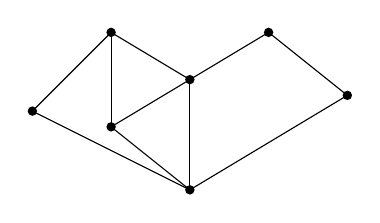
\begin{tikzpicture}[scale=1]
            \coordinate (a) at (-2,0);
            \coordinate (b) at (-1,1);
            \coordinate (c) at (0,0.4);
            \coordinate (d) at (1,1);
            \coordinate (e) at (2,0.2);
            \coordinate (f) at (0,-1);
            \coordinate (g) at (-1,-0.2);

            \draw (a)--(b)--(c)--(d)--(e)--(f)--(a);
            \draw (g)--(b);
            \draw (g)--(c);
            \draw (g)--(f);
            \draw (c)--(f);

            \foreach \p in {a,b,c,d,e,f,g}{
                \fill (\p) circle (1.7pt);
            }
        \end{tikzpicture}
    \]
\end{snippet}

\begin{snippetdefinition}{walk-length-definition}{Length of a walk}
    Let
    \[
        W=v_0,e_1,v_1,\ldots,e_n,v_n
    \]
    be a \walk in a \graph \(G\). The \emph{length} of \(W\) is the number
    \(n\) of edges occurring in the walk, counted with repetition.
\end{snippetdefinition}

\section{Connectedness}

\begin{snippetdefinition}{connected-vertices-definition}{Connected vertices}
    Let \(G\) be a \graph and let \(u,v\in V(G)\).
    The vertices \(u\) and \(v\) are \emph{connected} if there exists a
    \walk in \(G\) with origin \(u\) and terminal vertex \(v\).
    The empty walk is allowed, so every vertex is connected to itself.
\end{snippetdefinition}

\begin{snippetproposition}{walk-to-path-proposition}{Connected vertices are joined by a path}
    Let \(G\) be a \graph and let \(u,v\in V(G)\).
    If \(u\) and \(v\) are connected, then there exists a \path in \(G\)
    from \(u\) to \(v\).
\end{snippetproposition}

\begin{snippetproof}{walk-to-path-proof}{walk-to-path-proposition}{Connected vertices are joined by a path}
    Let
    \[
        v_0,e_1,v_1,\ldots,e_n,v_n
    \]
    be a walk from \(u=v_0\) to \(v=v_n\).
    If no vertex is repeated, the walk is already a path.
    Otherwise there exist indices \(i<j\) such that \(v_i=v_j\). Delete the
    closed part
    \[
        v_i,e_{i+1},v_{i+1},\ldots,e_j,v_j
    \]
    from the walk. The result is still a walk from \(u\) to \(v\), but it is
    shorter.

    Repeating this deletion process, after finitely many steps no repeated
    vertices remain. The resulting walk is a path from \(u\) to \(v\).
\end{snippetproof}

\begin{snippetdefinition}{graph-distance-definition}{Distance between vertices}
    Let \(G\) be a \graph and let \(u,v\in V(G)\) be connected vertices.
    The \emph{distance} between \(u\) and \(v\), denoted \(d(u,v)\), is the
    minimum length of a \walk joining \(u\) and \(v\).
    Every walk of minimum length is a path.
\end{snippetdefinition}

\begin{snippetdefinition}{connected-graph-definition}{Connected graph}
    A \graph \(G\) is \emph{connected} if every pair of vertices
    \(u,v\in V(G)\) is connected.
\end{snippetdefinition}

\begin{snippetproposition}{graph-connectedness-equivalence-relation}{Vertex connectedness is an equivalence relation}
    Let \(G\) be a \graph. The relation on \(V(G)\) defined by
    \[
        u\sim v
        \quad\Longleftrightarrow\quad
        u \text{ and } v \text{ are connected}
    \]
    is an \equivrelation.
\end{snippetproposition}

\begin{snippetproof}{graph-connectedness-equivalence-relation-proof}{graph-connectedness-equivalence-relation}{Vertex connectedness is an equivalence relation}
    The relation is reflexive because the empty walk connects every vertex to
    itself. It is symmetric because every walk can be traversed in the opposite
    direction. It is transitive because a walk from \(u\) to \(v\) followed by
    a walk from \(v\) to \(w\) gives a walk from \(u\) to \(w\).
\end{snippetproof}

\begin{snippetdefinition}{connected-components-definition}{Connected components}
    Let \(G\) be a \graph.
    The \emph{connected components} of \(G\) are the maximal connected
    subgraphs of \(G\). Equivalently, they are the equivalence classes of the
    connectedness relation on \(V(G)\), together with all edges whose endpoints
    lie in the same class.
\end{snippetdefinition}

\end{document}
